\chapter{Η Υλοποίηση της Κβαντικής Αριθμητικής Λογικής Μονάδας}

\section{Ο Ημι-Αθροιστής}
Για να υλοποιήσουμε κυκλώματα που τελούν πράξεις πρέπει να έχουμε ορίσει σωστά
το πώς τελούνται αυτές. Γνωρίζουμε ήδη ότι στην πρόσθεση, τα ψηφία των αριθμών
προστήθονται για να δώσουν το \emph{άθροισμα} τους. Την πράξη μπορούμε να τη
σκεφτούμε και να την τελέσουμε με τον παρακάτω τρόπο.\\

Θέλουμε έστω να προσθέσουμε τους δεκαδικούς αριθμούς $1$ και $2$.
Τοποθετούμε το κάθε ψηφίο των αριθμών το ένα κάτω από το άλλο, σε στοίλες.
Αφού το κάνουμε αυτό τελούμε την πρόσθεση με τους ήδη γνωστούς από το σχολειό
κανόνες της αριθμητικής.

\begin{table}
    \centering
    \begin{tabular}{c@{\,}c}
        & 1 \\
      + & 2 \\
      \hline
        & 3 \\
    \end{tabular}
    \label{tab:simple_decimal_addition}
    \caption{Η κλασική πράξη της πρόσθεσης σε μορφή αθροίσματος κατά στοίλες}
\end{table}


Αυτή η πράξη εκφράζεται $1 + 2 = 3$ και είναι ο τρόπος που περισσότερο
χρησιμοποιείται για τον συμβολισμό των πράξεων στον γραπτό λόγο.\\

Το κύκλωμα που θέλουμε να υλοποιήσουμε είναι ένα κύκλωμα το οποίο θα
προσθέτει δυο αριθμούς και στην έξοδο του θα δείνει το άθροισμα τους.

\subsubsection{Ο κλασικός ημι-αθροιστής}
Ο ημι-αθροιστής είναι ένα λογικό κύκλωμα το οποίο υπολογίζει
το άθροισμα $S$ (sum) καθώς και το πιθανό κρατούμενο $C$ (carry)
που μπορεί να προκύψει από την πρόσθεση δυο bit εισόδου $a, b$.
Για να υπολογίσουμε το άθροισμα $S$ των δυο δυαδικών ψηφίων εισόδου $a, b$ πρέπει
το κύκλωμα να παράγει στην έξοδο του $1$ μονό όταν ένα από τα δυο ψηφία είναι
ίσο με $1$. Αυτό μπορεί να υλοποιηθεί με τον λογικό τελεστή της αποκλειστικής σύζευξης,
ή εν συντομία XOR.

\begin{table}[ht]
    \centering
    \begin{tabular}{c c|c}
        $a$ & $b$ & $a \oplus b$ \\
        \hline
        0 & 0 & 0 \\
        0 & 1 & 1 \\
        1 & 0 & 1 \\
        1 & 1 & 0 \\
    \end{tabular}
    \label{tab:truth_tab_xor_gate}
    \caption{Ο πίνακας αληθείας της κλασικής λογικής πύλης XOR}
\end{table}

Για τον υπολογισμό του κρατουμένου $C$ πρέπει το κύκλωμα να παράγει στην
έξοδο του $1$ αν και μόνο αν $a = b = 1$. Αυτή η έκφραση μπορεί να
υλοποιηθεί με τον τελεστή σύζευξης ΚΑΙ (AND).

\begin{table}[ht]
    \centering
    \begin{tabular}{c c|c}
        $a$ & $b$ & $a \cdot b = a \land b$ \\
        \hline
        0 & 0 & 0 \\
        0 & 1 & 0 \\
        1 & 0 & 0 \\
        1 & 1 & 1 \\
    \end{tabular}
    \label{tab:truth_table_and_gate}
    \caption{Ο πίνακας αληθείας της κλασικής λογικής πύλης AND}
\end{table}

Γνωρίζοντας τα επιμέρους κομμάτια μπορούμε να κατασκευάσουμε το παρακάτω
κλασικό λογικό κύκλωμα για τον ημι-αθροιστή.

\begin{figure}[ht]
    \centering
    \begin{circuitikz}
        \draw (0, 4)node[xor port] (xorone){}
        (0, 2)node[and port] (and){}
        (xorone.in 1) node[left=1cm](a) {$a$}
        (xorone.in 2) node[left=1cm](b) {$b$}
        (xorone.out) node[right=0.1cm](s) {$S = a \oplus b$}
        (and.out) node[right=0.1cm](c) {$C = a \cdot b$}
        
        (a.east) to[short,-*] (xorone.in 1) |- (and.in 1)
        (b.east) to[short,-*] ($(b.east)!.5!(xorone.in 2)$) coordinate (branch)
        -- (xorone.in 2)
        (branch) |- (and.in 2);  
    \end{circuitikz}
    \label{fig:truth_table_halfadder}
    \caption{Το διάγραμμα του κλασικού κυκλώματος του ημι-αθροιστή}
\end{figure}

\begin{table}[ht]
    \centering
    \begin{tabular}{c c|c c}
        $a$ & $b$ & $S = a \oplus b$ & $C = a \cdot b$ \\
        \hline
        0 & 0 & 0 & 0 \\
        0 & 1 & 1 & 0 \\
        1 & 0 & 1 & 0 \\
        1 & 1 & 0 & 1 \\
    \end{tabular}
    \label{tab:truth_table_halfadder}
    \caption{Ο πίνακας αληθείας του κλασικού κυκλώματος του ημι-αθροιστή}
\end{table}

\subsubsection{Ο κβαντικός ημι-αθροιστής}
Για την υλοποίησει του κβαντικού ανάλογου του ημι-αθροιστή το μόνο που
χρειάζεται να κάνουμε είναι να αντιστοιχήσουμε τις βασικές λογικές πράξεις
με τις ανάλογες κβαντικές.\\
Η λογική πύλη AND αντιστοιχεί πλήρως με την κβαντική πύλη Toffoli. Αυτό μπορούμε
να το αποδείξουμε πολύ εύκολα σχεδιάζοντας τον πίνακα αληθείας τής.

\begin{figure}[ht]
    \centering
    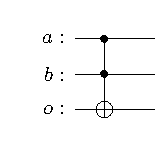
\includegraphics{images/3_Implementation_of_the_QALU/toffoli_gate_diagram.pdf}
    \label{fig:toffoli_gate_diagram}
    \caption{Το διάγραμμα της κβαντικής πύλης Toffoli}
\end{figure}

\begin{table}[ht]
    \centering
    \begin{tabular}{c c c|c c c}
        $a$ & $b$ & $o$ & $a'$ & $b'$ & $o'$ \\
        \hline
        0 & 0 & 0 & 0 & 0 & 0 \\
        0 & 1 & 0 & 0 & 1 & 0 \\
        1 & 0 & 0 & 1 & 0 & 0 \\
        1 & 1 & 0 & 1 & 1 & 1 \\
    \end{tabular}
    \label{tab:truth_table_toffoli}
    \caption{Ο πίνακας αληθείας της κβαντική πύλης Toffoli}
\end{table}

Όπως μπορούμε να διακρύνουμε οι πίνακες αληθείας είναι πανομοιότυποι με
αυτή της κλασικής πύλης AND. Επίσης το κβαντικό ανάλογο της κλασικής πύλης
XOR είναι η πύλη Feynman.

\begin{figure}[ht]
    \centering
    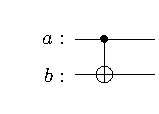
\includegraphics{images/3_Implementation_of_the_QALU/feynman_gate_diagram.pdf}
    \label{fig:feynman_gate_diagram}
    \caption{Το διάγραμμα της κβαντικής πύλης Feynman}
\end{figure}

\begin{table}[ht]
    \centering
    \begin{tabular}{c c|c c}
        $a$ & $b$ & $a'$ & $b'$ \\
        \hline
        0 & 0 & 0 & 0 \\
        0 & 1 & 0 & 1 \\
        1 & 0 & 1 & 1 \\
        1 & 1 & 1 & 0 \\
    \end{tabular}
    \label{tab:truth_table_feynman}
    \caption{Ο πίνακας αληθείας της κβαντική πύλης Feynman}
\end{table}

Γνωρίζοντας το πώς λειτουργεί ο κλασικός ημι-αθροιστής
μπορούμε να συνθέσουμε με ευκολία τον κβαντικό ημι-αθροιστή.
Έστω τα qubit εισόδου $\ket{a} = \ket{b} = \ket{0}$, θα χρειαστούμε
ένα βοηθητικό qubit $\ket{o} = \ket{0}$ το οποίο θα χρειαστεί για
τον υπολογισμό του κρατουμένου $\ket{C}$.\\

Αρχικά θα εφαρμόσουμε την πύλη Toffoli με qubit ελέγχου τα qubits
$\ket{a}, \ket{b}$ και το qubit στόχου το $\ket{o}$. Αυτή η ενέργεια
ισοδυναμεί με την λογική έκφραση $a \oplus b = C$.\\

Στο επόμενο βήμα θα εφαρμόσουμε την πύλη Feynman, με qubit-ελέγχου
το $\ket{a}$ και qubit-στόχο το $\ket{b}$. Αυτή η ενέργεια
ισοδυναμεί με την λογική έκφραση $a \cdot b = S$. Θέλουμε να επισημάνουμε
ότι αυτή η ενέργεια αλλάζει την κατάσταση του $\ket{b}_{new} = \ket{a} \cdot \ket{b}_{old}$.\\

\begin{figure}[ht]
    \centering
    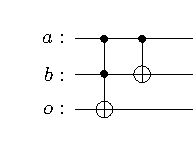
\includegraphics{images/3_Implementation_of_the_QALU/half_adder.pdf}
    \label{fig:quantum_halfadder_diagram}
    \caption{Το διάγραμμα του κβαντικού-λογικού κυκλώματος του ημι-αθροιστή}
\end{figure}

\section{Ο Πλήρης Αθροιστής}

Όπως δείξαμε στο προηγούμενο κεφάλαιο, κατά την πρόσθεση δυο αριθμών,
έχουμε μάθει να προσθέτουμε τα ψηφία των αριθμών - το ένα μετά το άλλο
εώς ότου εξαντλήσουμε τα ψηφία. Βέβαια, κατά την πρόσθεση δύο, ψηφίων
μπορεί το άθροισμα τους να είναι μεγαλύτερο του δέκα. Έχουμε μάθει σε
αυτή τη περίπτωση, να γράφουμε το λιγότερο σημαντικό του αθροίσματος,
σαν ψηφίο τους τελικού αθροίσματος, και το σημαντικότερο ψηφίο ως κρατούμενο
για την επόμενη πράξη.

\begin{table}[ht]
    \centering
    \begin{tabular}{c@{\,}c@{\,}c}
          & 1 &   \\
          & 1 & 2 \\
        + &   & 9 \\
        \hline
          & 2 & 1 \\
    \end{tabular}
    \label{tab:simple_decimal_addition_wcarry}
    \caption{Μια απλή πράξη πρόσθεσης με δημιουργία κρατουμένου}
\end{table}

Στο παράπανω παράδειγμα, κατά την πρόσθεση των λιγότερο σημαντικών ψηφίων
των αριθμών $12$ και $9$, δημιούργηθηκε αποτέλεσματα μεγαλύτερο του δέκα
($2 + 9 = 11$) άρα γράφουμε, ένα ($1$) στο αποτέλεσμα και το ένα ($1$) στο κρατούμενο
το οποίο θα χρησιμοποιηθεί στο επόμενο σκέλος. Στο τελευταίο σκέλος της πράξης έχουμε
απλά να προσθέσουμε το κρατούμενο ($1$) με τα σημαντικότερα ψηφία ($1$ και, νοητά, $0$)
των αριθμών $12$ και $9$. Σε αυτό το κεφάλαιο θα χρησιμοποιήσουμε τα λογικά, κλασικά και
κβαντικά κυκλώματα με σκοπό την υλοποιήσει της παραπάνω αριθμητικής πράξης.\\

Το κύκλωμα που υλοποιεί την πράξη της πρόσθεσης λαμβάνοντας υπόψιν κρατούμενο από
κάποια προηγούμενη πρόσθεση ονομάζεται \emph{πλήρης αθροιστής}. Ό λόγος που αυτό το κύκλωμα
χαρακτηρίζεται ως \say{πλήρες} είναι δύο. Πρώτον, χρησιμοποιεί δυο ημι-αθροιστές
για την υλοποίηση των λειτουργειών του, και δεύτερον, όπως είχαμε αναφέρει και
παραπάνω, το κύκλωμα λαμβάνει υπόψιν πιθανό κρατούμενο από προηγούμενη πράξη και
άρα υλοποιεί πλήρως την πράξης της πρόσθεσης. Πως όμως λειτουργεί η πλήρης πρόσθεση
στο δυαδικό σύστημα;\\

Ας αρχισόυμε με ένα απλό παράδειγμα. Θα τελέσουμε την πρόσθεση των αριθμών
$12 + 9$. (Για να μπορέσουμε να προσεγγίσουμε καλύτερα την λειτουργεία του πλήρη αθροιστής
θα υποθέσουμε οτι οι αριθμοί θα κωδικοποιήθουν ως απροσήμαστοι δυαδικοί  αριθμοί.)
Αρχικά κωδικοποιούμε τους αριθμούς μας στο δυαδικό σύστημα, $12_{10} \mapsto 1100_2$ και
$9_{10} \mapsto 1001_2$. Μετά θα στοιχήσουμε τα δυαδικά ψηφία των αριθμών με τον γνωστό τρόπο
της πρόσθεση κατά στοίλες. Τέλος θα ακολουθήσουμε τους εξής κανόνες:

\begin{enumerate}
  \item $0 + 0 = 0$
  \item $0 + 1 = 1 + 0 = 1$
  \item $1 + 1 = 10$, όπου το σημαντικότερο ψηφίο ($1$) θα γραφεί
  πάνω από τα ψηφία της επόμενης πράξης και το λιγότερο σημαντικό ($0$)
  στο αποτέλεσμα
  \item $1 + 1 + 1 = 11$, όπου το σημαντικότερο ψηφίο ($1$) θα γραφεί
  πάνω από τα ψηφία της επόμενης πράξης και το λιγότερο σημαντικό ($1$)
  στο αποτέλεσμα
\end{enumerate}

\begin{center}
  \begin{tabular}{c@{\,}c@{\,}c@{\,}c@{\,}c}
    1 &   &   &   &   \\
      & 1 & 1 & 0 & 0 \\
    + & 1 & 0 & 0 & 1 \\
    \hline
    1 & 0 & 1 & 0 & 1 \\
    \end{tabular}
\end{center}

Όπως μπορούμε να δούμε, το αποτέλεσμα της πράξης $1100_2 + 1001_2 = 10101_2 \mapsto 21_{10}$
είναι αυτό που περιμέναμε.

\subsection{Ο κλασικός πλήρης αθροιστής}

Θα προσπαθήσουμε να συστηματοποιήσουμε το παραπάνω παράδειγμα. Έστω τρια
bit εισόδου για τον πλήρη αθροιστή $a, b, c_{in}$. Τα $a, b$ είναι τα bit
των αριθμών και το $c_{in}$ το κρατούμενο εισόδου, δηλαδή το κρατούμενο από
μια προηγούμενη πιθανή πρόσθεση. Θέλουμε το κύκλωμα να βγάζει ως άθροισμα
στην έξοδο $S = 1$ μόνο όταν $(a \oplus b) \oplus c_{in}$. Τέλος, θέλουμε
να βγάζει ως κρατούμενο στην έξοδο $C_{out}$ μόνο όταν $(a \oplus b) \cdot c_{in} + a \cdot b$.
Γνωρίζοντας τις δύο προηγούμενες εξισώσεις μπορούμε να συνθέσουμε το κλασικό
κύκλωμα του πλήρη αθροιστή.\\

\begin{figure}[ht]
  \centering
  \begin{circuitikz}
      \draw (7.5,13.75) to[short] (8,13.75);
      \draw (7.5,13.25) to[short] (8,13.25);
      \draw (8,13.75) node[xor port, anchor=in 1, scale=0.89](port){} (port.out) to[short] (10,13.5);
      \draw (12.75,13.5) to[short] (13.25,13.5);
      \draw (12.75,13) to[short] (13.25,13);
      \draw (13.25,13.5) node[xor port, anchor=in 1, scale=0.89](port){} (port.out) to[short] (15.25,13.25);
      \draw (7.5,11.75) to[short] (8,11.75);
      \draw (7.5,11.25) to[short] (8,11.25);
      \draw (8,11.75) node[and port, anchor=in 1, scale=0.89](port){} (port.out) to[short] (10,11.5);
      \draw (12.75,11.5) to[short] (13,11.5);
      \draw (12.75,11) to[short] (13,11);
      \draw (13,11.5) node[and port, anchor=in 1, scale=0.89](port){} (port.out) to[short] (15,11.25);
      \draw (16.25,11.25) to[short] (16.75,11.25);
      \draw (16.25,10.75) to[short] (16.75,10.75);
      \draw (16.75,11.25) node[or port, anchor=in 1, scale=0.89](port){} (port.out) to[short] (18.75,11);
      \draw[] (7.5,13.75) to[short] (6.25,13.75);
      \draw[] (7.5,13.25) to[short] (6.25,13.25);
      \draw [](7.5,13.75) to[short] (7.5,11.75);
      \draw [](7,13.25) to[short] (7,11.25);
      \draw (7.5,13.75) to[short, -*] (7.5,13.75);
      \draw (7,13.25) to[short, -*] (7,13.25);
      \node [font=\normalsize] at (6,13.75) {$a$};
      \node [font=\normalsize] at (6,13.25) {$b$};
      \node [font=\normalsize] at (6,9.5) {$c_{in}$};
      \node [font=\normalsize] at (19,13.25) {$S$};
      \node [font=\normalsize] at (19.25,11) {$C_{out}$};
      \draw[] (7.5,11.25) to[short] (7,11.25);
      \draw [](10,13.5) to[short] (12.75,13.5);
      \draw [](11.75,13.5) to[short] (11.75,11.5);
      \draw [](11.75,11.5) to[short] (12.75,11.5);
      \draw (11.75,13.5) to[short, -*] (11.75,13.5);
      \draw [](15.25,13.25) to[short] (18.75,13.25);
      \draw [](15,11.25) to[short] (16.25,11.25);
      \draw[] (12.75,13) to[short] (11,13);
      \draw [](11,13) to[short] (11,9.5);
      \draw [](6.25,9.5) to[short] (11,9.5);
      \draw [](10,10) to[short] (16.25,10);
      \draw [](16.25,10) to[short] (16.25,10.75);
      \draw[] (12.75,11) to[short] (11,11);
      \draw (11,11) to[short, -*] (11,11);
      \draw [](10,11.5) to[short] (10,10);
      \draw [, dashed] (6.5,14.25) rectangle  (10.5,10.5);
      \draw [, dashed] (11.25,14.25) rectangle  (15.25,10.5);
  \end{circuitikz}
  \label{fig:10}
  \caption{Το κλασικό κύκλωμα του πλήρη αθροιστή}
\end{figure}

\begin{figure}[ht]
  \centering
  \begin{tabular}{c c c|c c}
    $a$ & $b$ & $c_{in}$ & $S$ & $C_{out}$ \\
    \hline
    $0$ & $0$ & $0$ & $0$ & $0$ \\
    $0$ & $1$ & $0$ & $1$ & $0$ \\
    $1$ & $0$ & $0$ & $1$ & $0$ \\
    $1$ & $1$ & $0$ & $0$ & $1$ \\
    $0$ & $0$ & $1$ & $1$ & $0$ \\
    $0$ & $1$ & $1$ & $0$ & $1$ \\
    $1$ & $0$ & $1$ & $0$ & $1$ \\
    $1$ & $1$ & $1$ & $1$ & $1$ \\
  \end{tabular}
  \label{fig:11}
  \caption{Ο πίνακας αληθείας του κλασικού κυκλώματος του πλήρη αθροιστή}
\end{figure}

\subsection{Ο κβαντικός πλήρης αθροιστής}

Με βάση των κλασικό πλήρη αθροιστή και των κβαντικό ημι-αθροιστή
μπορούμε με σχετική ευκολία να συνθέσουμε των κβαντικό πλήρη
αθροιστή.\\

Ο κβαντικός πλήρης αθροιστής είναι ένα κβαντικό κύκλωμα το οποίο
λαμβάνει τέσσερα qubit στις εισόδους $\ket{a}, \ket{b}, \ket{c_{in}}$
και $\ket{d}$ τα όποια μετασχηματίζονται έτσι ώστε να ισχύει:
$\ket{a \otimes b \otimes c_{in} \otimes d} \mapsto \ket{a \otimes b \otimes S \otimes C_{out}}$.
Με απλά λόγια, ο κβαντικός πλήρης αθροιστής μετασχηματίζει τα qubit 
$\ket{c_{in}}$ και $\ket{d}$ με τέτοιο τρόπο ώστε στο τέλος των υπολογισμών
το $\ket{c_{in}}$ να περιέχει το άθροισμα $\ket{a+b+c_{in}} = \ket{S}$ και το $\ket{d}$ να περιέχει το κρατόυμενο
της πρόσθεσης.\\

Αναλύοντας το ζητούμενο, μπορούμε με ευκολία να καταγράψουμε
τον πίνακα αληθείας του κβαντικού πλήρη αθροιστή.

\begin{figure}[ht]
  \centering
  \begin{tabular}{c c c c|c c c c}
    $a$ & $b$ & $c_{in}$ & $d$ & $a$ & $b$ & $S$ & $C_{out}$ \\
    \hline
    $0$ & $0$ & $0$ & $0$ & $0$ & $0$ & $0$ & $0$ \\
    $0$ & $1$ & $0$ & $0$ & $0$ & $1$ & $1$ & $0$ \\
    $1$ & $0$ & $0$ & $0$ & $1$ & $0$ & $1$ & $0$ \\
    $1$ & $1$ & $0$ & $0$ & $1$ & $1$ & $0$ & $1$ \\
    $0$ & $0$ & $1$ & $0$ & $0$ & $0$ & $1$ & $0$ \\
    $0$ & $1$ & $1$ & $0$ & $0$ & $1$ & $0$ & $1$ \\
    $1$ & $0$ & $1$ & $0$ & $1$ & $0$ & $0$ & $1$ \\
    $1$ & $1$ & $1$ & $0$ & $1$ & $1$ & $1$ & $1$ \\
  \end{tabular}
  \label{fig:13}
  \caption{Ο πίνακας αληθείας του κλασικού κυκλώματος του πλήρη αθροιστή}
\end{figure}


Κατά το βήμα 1, το qubit $d$ μετασχηματίζεται έτσι ώστε $d' = a \cdot b$.

\begin{figure}[!ht]
  \centering
  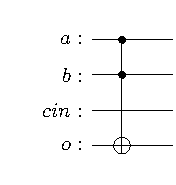
\includegraphics{images/3_Implementation_of_the_QALU/full_adder_step1.pdf}
  \label{fig:14}
  \caption{Βήμα 1: Του κβαντικού πλήρη αθροιστή}
\end{figure}

Κατά το βήμα 2, το qubit $b$ μετασχηματίζεται έτσι ώστε $b' = a \oplus b$.

\begin{figure}[!ht]
  \centering
  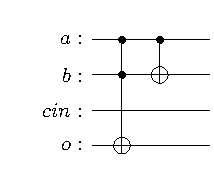
\includegraphics{images/3_Implementation_of_the_QALU/full_adder_step2.pdf}
  \label{fig:15}
  \caption{Βήμα 2: Του κβαντικού πλήρη αθροιστή}
\end{figure}

Κατά το βήμα 3, το qubit $d'$ μετασχηματίζεται έτσι ώστε $d'' = (ab) + (a \oplus b)c_{in}$.
Μετά από αυτό το βήμα το qubit $d''$ θα περιέχει το κρατούμενο της πρόσθεσης $a + b + c_{in}$.

\begin{figure}[!ht]
  \centering
  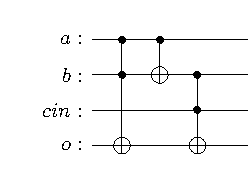
\includegraphics{images/3_Implementation_of_the_QALU/full_adder_step3.pdf}
  \label{fig:16}
  \caption{Βήμα 3: Του κβαντικού πλήρη αθροιστή}
\end{figure}

Κατά το βήμα 4, το qubit $c$ μετασχηματίζεται έτσι ώστε $c' = a \oplus b \oplus c_{in}$.
Μετά από αυτό το βήμα το qubit $c'$ θα περιέχει το άθροισμα της πρόσθεσης $a + b + c_{in}$.

\begin{figure}[!ht]
  \centering
  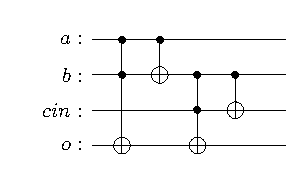
\includegraphics{images/3_Implementation_of_the_QALU/full_adder_step4.pdf}
  \label{fig:17}
  \caption{Βήμα 4: Του κβαντικού πλήρη αθροιστή}
\end{figure}

Τέλος, στο βήμα 5, επαναφέρουμε το qubit $b'$ στην αρχική του κατάσταση δρώντας πάνω του
ξανά με την πύλη Tofolli ελεγχόμενη από το qubit $a$.

\begin{figure}[!ht]
  \centering
  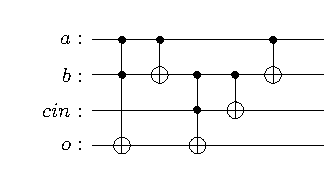
\includegraphics{images/3_Implementation_of_the_QALU/full_adder.pdf}
  \label{fig:18}
  \caption{Το διάγραμμα του κβαντικού-λογικού κυκλώματος του πλήρη αθροιστή}
\end{figure}

\section{Ο Αθροιστής-Αφαιρέτης}
\section{Ο Πολλαπλασιαστής Ακεραίων}
\section{Ο Συγκριτής Αριθμητικών Μεγεθών}